\documentclass[10pt]{article}
\usepackage[utf8]{inputenc}
\usepackage[OT1]{fontenc}
\usepackage{amsfonts, amsmath, amsthm, amssymb}
\usepackage{bbm}
\usepackage{mathtools}
\usepackage{natbib}
\usepackage{graphicx}
\usepackage{listings}
\usepackage[margin=1in]{geometry}
\usepackage{xcolor}
\usepackage{bigints}
\usepackage{glossaries}
\usepackage{graphicx}
% \graphicspath{ {./images/} }

\theoremstyle{definition}
\newtheorem{definition}{Definition}[section]

\newtheorem{theorem}{Theorem}

\newcounter{countCode}
\lstnewenvironment{code} [1][caption=Ponme caption, label=default]{%
	\renewcommand*{\lstlistingname}{Listado} 
	\setcounter{lstlisting}{\value{countCode}} 
	\lstset{ %
	language=java,
	basicstyle=\ttfamily\footnotesize,       % the size of the fonts that are used for the code
	numbers=left,                   % where to put the line-numbers
	numberstyle=\sc,      % the size of the fonts that are used for the line-numbers
	stepnumber=1,                   % the step between two line-numbers. 
	numbersep=5pt,                 % how far the line-numbers are from the code
	numberstyle=\color{red!50!blue},
    	backgroundcolor=\color{lightgray!20},
	rulecolor=\color{blue},
	keywordstyle=\color{red}\bfseries,
	showspaces=false,               % show spaces adding particular underscores
	showstringspaces=false,         % underline spaces within strings
	showtabs=false,                 % show tabs within strings adding particular underscores
	frame=single,                   % adds a frame around the code
	framexleftmargin=0mm,
	numberblanklines=false,
	xleftmargin=5pt,
	breaklines=true,
	breakatwhitespace=true,
	breakautoindent=true,
	captionpos=t,
	texcl=true,
	tabsize=2,                      % sets default tabsize to 3 spaces
	extendedchars=true,
	inputencoding=utf8, 
	escapechar=\%,
	morekeywords={print, println, size, background, strokeWeight, fill, line, rect, ellipse, triangle, arc, save, PI, HALF_PI, QUARTER_PI, TAU, TWO_PI, width, height,},
	emph=[1]{print,println,}, emphstyle=[1]{\color{blue}}, % Mis palabras clave.
	emph=[2]{width,height,}, emphstyle=[2]{\bf\color{violet}}, % Mis palabras clave.
	emph=[3]{PI, HALF_PI, QUARTER_PI, TAU, TWO_PI}, emphstyle=[3]\color{orange!50!violet}, % Mis palabras clave.
	emph=[4]{line, rect, ellipse, triangle, arc,}, emphstyle=[4]\color{green!70!black}, % Mis palabras clave.
	%emph=[5]{size, background, strokeWeight, fill,}, emphstyle=[5]{\tt \color{red!30!blue}}, % Mis palabras clave.
	%emph={[2]sqrt,baset}, emphstyle={[2]\color{blue}}, % f(sqrt(2)), sqrt a nivel 2 se pondrá azul
	#1}}{\addtocounter{countCode}{1}}



\title{Probability \& Optimal Transport}
\author{Davi Sales Barreira}
\date{\today}
\begin{document}
\maketitle \tableofcontents 


\begin{abstract}
The main goal of these notes is to present an introduction to the transport inequalities,
which consist of methods of using Optimal Transport Theory to obtain concentration
inequalities in high-dimensional probability. Along the way, as new concepts are presented,
some side-lining will be done, with the aim to explore some of these new concepts, before
diving back in the proof of the inequalities. The core of these notes are base on the
excellent paper "Transport Inequalities. A Survey" by \cite{gozlan2010transport}.
\end{abstract}

% \section*{Notation}
% \begin{itemize}
% 	\item $P(\mathcal X)$ - S
% 	Most of the content regarding transportation inequality is from
% \end{itemize}

\section{introduction}
Given two probability distributions $\mu,\nu$, there are many situations
where one is interested in defining a way of measuring the
distance between them. The Wasserstein distance is a
metric that arises from the idea of optimal transport, and which has being
gaining attention in Statistics and Machine Learning. One prominent example is the so
called Wasserstein Generative Adversarial Network (WGAN), which uses this metric to evaluate
how well the model generated distribution approximates the "real" distribution of the
data. As will be shown shortly, the Wasserstein metric has several advantages compared to
other metrics.

There are several ways of defining distances between two
probability measures. Let's assume that $\nu, \mu$ are defined on 
$(\Omega, \mathcal F)$ and that $\nu \ll \lambda$,
$\mu \ll \lambda$ , for $\lambda$ representing the Lebesgue measure. Below
we present some example of distances:

\begin{align*} 
\text{Total Variation} &: \quad || \mu - \nu ||_{TV} =
\sup_{A \in \mathcal F} |\mu (A) - \nu(A)| = 
\frac{1}{2}\int_\Omega \left | \frac{d\mu}{d\lambda} - \frac{d\nu}{d\lambda} \right
|d\lambda
= \sup_{|f|\leq 1} \left |
\int f (d\nu - d\mu)\right|
\\
\\
\text{Hellinger} &: \quad \sqrt{\bigintss_\Omega \left(\sqrt{\frac{d\mu}{d\lambda}} -
\sqrt{\frac{d\nu}{d\lambda}} \right )^2d\lambda} \\
\\
L_2 &: \quad \int_\Omega \left(\frac{d\mu}{d\lambda} - \frac{d\nu}{d\lambda}\right)^2
d\lambda \\
% \text{Relative Entropy} &: \quad
% H(\nu \mid \mu) =
% \left\{
%   \begin{array}{@{}ll@{}}
%     \int_\mathcal X \log(\frac{d\nu}{d\mu})d\nu, & \text{if}\ \nu \ll\mu \\
%     +\infty, & \text{otherwise}
%   \end{array}\right.
%   \\
%   \\
\end{align*}

As pointed out by \citet{wassermanStatisicalMethods2018} in his lecture notes,
although such distances are useful, there are drawbacks:
\begin{itemize}
	\item If one distribution is discrete and the other is continuous,  they cannot
	be compared. If $X \sim U(0,1)$ and $Y$ is uniform on $\{0,1/N, 2/N,...,1\}$,
	although this distributions are very similar, their total variation is 1 (which is
	the maximum value). The Wasserstein distance is $1/N$, which is reasonable.
	\item These distances ignore the "geometry of the underlying space", while the
	Wasserstein distance preserves it, as shown in Figure~\ref{fig:distances}.
	\item When "averaging" different distributions, one might be interested in obtaining
	a similar distribution, avoiding smoothing. This can be done using the Wasserstein
	barycenter, as shown in Figure~\ref{fig:barycenter}.
\end{itemize}
\begin{figure}[h]
	\centering
	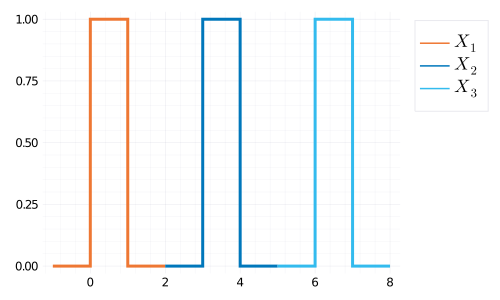
\includegraphics[width=8cm]{images/Distributions_Distances.png}
    \caption{Each pair has the same distance in $L_2$, Hellinger and TV. But using
    Wasserstein, $X_1$ is closer to $X_2$ than to $X_3$.}
    \label{fig:distances}
\end{figure}

\begin{figure}[h]
	\centering
	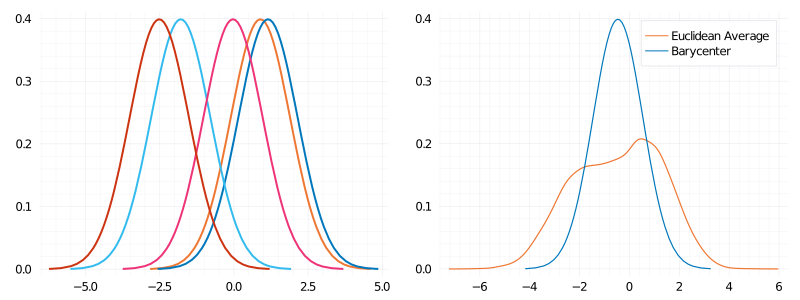
\includegraphics[width=14cm]{images/Barycenter.png}
    \caption{In the left you have different distributions, and in the right,
    there is a comparison between averaging these distribution versus finding the
    Wasserstein barycenter.}
    \label{fig:barycenter}
\end{figure}

\section{Optimal Transport and the Wasserstein Distance}

Let $\mathcal X$ be a polish space, and define a function
$c: \mathcal X \times \mathcal X \rightarrow [0,\infty)$, where $c$ is a lower semicontinuous function and $\mu,\nu \in P(\mathcal)$ (this means that $\mu$ and $\nu$ are
probability measures on $X$). Function $c$ is usually called the \textit{cost function}.
The Wasserstein distance arises from the Monge-Kantorovich optimal transport problem, which
seeks to find a map
$\pi: \mathcal X \times \mathcal X \rightarrow \mathcal X \times \mathcal X$, that
transport $\mu$ to $\nu$ with minimum cost.

\theoremstyle{definition}
\begin{definition}{Coupling}
A probability measure $\pi \in P(\mathcal X \times \mathcal Y)$ is called a coupling of
$\mu \in P(\mathcal X)$ and $\nu \in P(\mathcal Y)$ if it's marginal distributions
$\pi_1$ and $\pi_2$ are
$\mu$ and $\nu$.
\end{definition}

\begin{equation*}
	(MK) \quad \text{Minimize} \pi \in P(\mathcal X^2) \mapsto
	\int_{\mathcal X^2} c(x,y) d\pi(x,y) \ \text{subject to } \pi
	\text{coupling of } (\nu,\mu)
\end{equation*}

From solving the above problem, one obtains the optimal transport cost, given by:
\begin{equation}
	T_c(\nu, \mu) :=
	\inf \left\{
		\int_{\mathcal X^2} c(x,y) d\pi(x,y) \ ; \pi_1 = \nu, \pi_2 = \mu
	\right\}
\end{equation}

Now, given a metric space $(\mathcal X, d)$, we say that $f: \mathcal X \rightarrow \mathbb R$
is $L$-Lipschitz if
\begin{equation}
	\mid f(x) - f(y) \mid \leq L d(x,y) \quad \forall x,y \in \mathcal X
\end{equation}

We will use $||f||_{Lip}$ to denote the smallest $L$ for which this inequality holds.
Also, denote $P_1(\mathcal X)$ the space of probability measures with finite first moment.

Therefore, for $\mu,\nu \in P_1(\mathcal X)$, the Wasserstein distance is then defined as 
$$
W_d(\nu, \mu) := \sup_{||f||_{Lip}\leq 1} \left |
\int f d\nu - \int f d\mu	
\right |
$$

A classical results in the optimal transport theory, called
\textit{Kantorovich-Rubinstein duality} (which will not be proved here),
guarantees the equivalence between the Wasserstein distance and the optimal transport cost
when the underlying metric space is separable.
Hence, by setting $c = d^p$ where , where $d$ is a metric
on $\mathcal X$ and $p \geq 1$,
\begin{equation}
W_{d^p}(\nu,\mu):= T_{d^p}(\nu,\mu)^{\frac{1}{p}}
\end{equation}

When the context allows, we will write $W_p$ instead of $W_{d^p}$. Note that depending on
the reference, the Wasserstein distance might be first defined as a transport cost. A
simple proof for this duality in the discrete setting 
is present in the lecture notes by \citet{van2014probability}.

Note that $W_p$ are proper metrics (positive, symmetric and satisfy the triangle inequality)
in the space of probability measures. Also, the spaces with $p$-th moments finite, the
metric space $(P_p(\mathcal X), W_p)$ is complete and separable if so is $\mathcal X$ \citep{panaretos2019statistical}. Hence, the Wasserstein distance has the interesting features
already presented, such as incorporating the geometry of the "ground space", and allowing
the comparison between discrete and continuous distributions. Another interesting aspect,
is that convergence of r.v $X_n$ to $X$ in $W_p$ distance is equivalent to convergence in
distribution with $E|X_n|^p \rightarrow E |X|^p$ \citep{panaretos2019statistical}.

\section{Transport Inequalities and Concentration}

In the literature, there are a range of different methods for obtaining inequalities
concerning the phenomenon of concentration of measure. The use of transport inequalities
is a more recent endeavor and usually not present in more basic texts concerning
high-dimensional probability, such as the book by \citet{vershynin2018high}.
The relation of optimal transport to concentration inequalities was first pointed out by \citet{marton1986simple},  and advanced through the nineties, with advances in optimal
transport theory. Take a look at \citet{gozlan2010transport} for a more complete overview
on the topic.

\begin{definition}[Transport Inequalities]
	Let $J(\cdot \mid \mu): P(\mathcal X)$ and
	$\alpha:[0,\infty) \rightarrow [0,\infty)$ an increasing function with $\alpha(0)=0$.
	One says that $\mu \in P(\mathcal X)$ satisfy the transport inequality
	$\alpha(T_c) \leq J$ if
	$$
	\alpha(T_c(\nu,\mu)) \leq J(\nu \mid \mu) , \quad \forall \nu \in P(\mathcal X)
	$$
\end{definition}
\begin{definition}[Relative Entropy]
$$
	H(\nu \mid \mu) =
	\left\{
	  \begin{array}{@{}ll@{}}
	    \int_\mathcal X \log(\frac{d\nu}{d\mu})d\nu =
	    \int_\mathcal X \frac{d\nu}{d\mu}\log(\frac{d\nu}{d\mu})d\mu
	    , & \text{if}\ \nu \ll\mu \\
	    +\infty, & \text{otherwise}
	  \end{array}\right.
$$
\end{definition}

When $J  = H$, one also calls these transport-entropy inequalities. Among the family
of transport inequalities, two classical ones are the $\textbf T_1$ and $\textbf T_2$. We
say that $\mu \in P_p(\mathcal X)
:= \{ \nu \in P(\mathcal X): \int d(x_o, \cdot)^p d\nu < \infty\}$ satisfies
$\textbf T_p(C)$, for $C > 0$ if

\begin{equation}
	W_p^2(\nu,\mu) \leq C H(\nu \mid \mu)
\end{equation}

Note that $\textbf T_1(C)$ is weaker than $\textbf T_2(C)$, because, if $\mu$ satisfies
$\textbf T_2(C)$, then
\begin{align*}
W_2^2(\nu,\mu) \leq C H(\nu \mid \mu) &\implies C^{-1}(T_{d^2}(\nu,\mu)^{1/2})^2 \leq H
\\
&\xRightarrow{Jensen}
C^{-1}(T_{d})^2(\nu,\mu) \leq 
C^{-1}T_{d^2}(\nu,\mu) \leq H(\nu \mid \mu)
\end{align*}

The following inequality is a classical result in information theory.
\begin{theorem}[Pinsker-Csiszár-Kullback inequality]
$$
|| \nu - \mu ||^2_{TV} \leq \frac{1}{2}H(\nu \mid \mu),
$$

for all $\mu,\nu \in P(\mathcal X)$.
\end{theorem}

\begin{proof}
	This proof is taken from \citet{gozlan2010transport} and is originally attributed
	to Talagrand. Suppose $H(\nu \mid \mu) < \infty$ (otherwise we are done). Let
	$f = \frac{d\nu}{d\mu}$ and $u = f - 1$, which implies $\int u d\mu = 0$
	$$
	H(\nu \mid \mu) = \int_\mathcal X f \log f d\mu  =
	\int_\mathcal X (1+u) \log(1+u) - u \ d\mu
	$$

	For $\phi(u) = (1+u)\log(1+u) - u$, one can do some manipulations to obtain:
	$$
	\phi(u) = \int_0^y \frac{(u-x)}{1+u} dx = u^2 \int^1_0 \frac{1-s}{1+su} ds,
	\quad u > -1
	$$

	Then, substituting in the relative entropy equation

	$$
	H(\nu \mid \mu) = \int_\mathcal X \phi(u) du  =
	\int_\mathcal X u^2
	\int_0^1 \frac{1-s}{1+su} \ ds \ d\mu =
	\int_{\mathcal X \times [0,1]} u(x)^2\frac{1-s}{1+su(x)} \ ds \ d\mu(x)
	$$

	We can rewrite some equations and apply Cauchy-Schwarz inequality, to obtain the
	following
	\begin{align*}
		\left(\int_{\mathcal X \times [0,1]} |u(x)|(1-s)d\mu(x) \ ds
		\right)^2
		&\leq 
		\int_{\mathcal X \times [0,1]} u(x)^2\frac{1-s}{1+su(x)} \mu(x) \ ds \ \cdot \\
		&\int_{\mathcal X \times [0,1]} (1-s)(1+su(x))d\mu(x) \ ds
	\end{align*}


	Noting that:
	\begin{align*}
		\int_{\mathcal X \times [0,1]} |u(x)|(1-s)d\mu(x) \ ds
		&=
		\frac{1}{2}\int_\mathcal X |1 - f| d\mu
		\\
		&= \frac{1}{2}\int_\mathcal X \left|\frac{d\mu}{d\mu} - \frac{d\nu}{d\mu}
		\right| d\mu = || \nu - \mu ||_{TV}
	\end{align*}
	And that
	\begin{align*}
		\int_{\mathcal X \times [0,1]} u(x)^2\frac{1-s}{1+su(x)} \mu(x) \ ds \ \cdot \int_{\mathcal X \times [0,1]} (1-s)(1+su(x))d\mu(x) \ ds = 
		H(\nu \mid \mu) \cdot \frac{1}{2}
	\end{align*}

	We conclude that
$$
|| \nu - \mu ||^2_{TV} \leq \frac{1}{2}H(\nu \mid \mu),
$$


\end{proof}

The connection with the transport cost is made by defining the Hamming metric
\begin{definition}[Hamming metric]
$$d_H(x,y) = \mathbbm 1_{x \neq y}, \quad x,y \in \mathcal X$$
\end{definition}

Now, observe that using $d_H$, then $|f(x) - f(y)| \leq d_H(x,y) \leq 1$, hence
\begin{equation}
W_{d_h}(\nu, \mu) = \sup_{|f|\leq 1} \left |
\int f d\nu - \int f d\mu	
\right | = || \mu - \nu ||_{TV}
\end{equation}

Using the Kantorovich-Rubinstein duality, one would then obtain that
$T_{d_H}(\mu,\nu) =|| \mu - \nu ||_{TV} $. The problem is that $(\mathcal X, d_H)$
is not separable, unless $\mathcal X$ is discrete. Fortunately, one can still prove
that indeed the duality is still valid for this metric. The proof for this assertion
is present in Example 4.14 at \citet{van2014probability}. Briefly, the proof consists
of explicitly constructing the optimal coupling, and showing that $|| \mu - \nu ||_{TV}$
coincides with $T_{d_H}(\nu,\mu)$.
Therefore, a probability measure $\mu$ defined in the metric space $(\mathcal X, d_H)$
satisfies the $\textbf T_1(1/2)$ inequality.

Before showing how this entails a
concentration inequality, one needs a little more results.

\begin{definition}[Concentration of measure]
For a metric space $(\mathcal X, d)$ and $r \geq 0$. The $r$-neighborhood of
$A \subset \mathcal X$ is

$$
A^r := \{
x \in \mathcal X: \ d(x,A) \leq r
\},
\quad d(x,A) := \inf_{y \in A} d(x,y)
$$

Hence, for $\beta: [0,\infty) \rightarrow \mathbb R_+$ such that $\beta(r) \rightarrow 0$
when $r \rightarrow \infty$. One says that the probability measure $\mu$ satisfies the
concentration inequality with profile $\beta$ if,
$$
\mu(A^r) \geq 1 - \beta(r)
$$
\end{definition}
for all measurable $A \in \mathcal X$ and $\mu(A) \geq 1/2$ .
% section  (end)

% \section*{References}
% \addcontentsline{toc}{section}{References}
  \bibliography{probability_ot}
  \bibliographystyle{plainnat}
  % \bibliographystyle{plainnat}
  % \bibliographystyle{plain}
  % \bibliographystyle{abbrv}
\end{document}

